\section{Princípios de Arquitetura Limpa}

    \par Esta seção tem como objetivo, explorar os conceitos da Arquitetura Limpa desde o seu surgimento no ano de 2012 até os mais recentes estudos na área e implementações feitas pelos autores citados nesse trabalho. Abordar os conceitos da Arquitetura Limpa é necessário para entender quais princípios ela prega e como vamos relaciona-los de maneira prática mais a frente nesse trabalho com o padrão arquitetural MVC.
    
    \subsection{Contexto histórico}
    
        \par A Arquitetura Limpa foi proposta por \cite{livro:martin:cleanarch} no ano de 2012, conforme publicado no blog The Clean Code Blog \cite{artigo:ferreira:2022}. A abordagem para criação desces princípios foi desenvolvida com base em sua experiência como programador desde 1970 \cite{livro:martin:cleanarch}.
        
        \par O surgimento da Arquitetura Limpa está associado à "crise do software" da década de 1960, caracterizada por problemas como prazos não cumpridos, custos elevados, baixa produtividade, qualidade insuficiente e dificuldades de manutenção em aplicações \cite{artigo:dantas:2021, artigo:ferreira:2022}. Essa crise evidenciou a necessidade de métodos para gerenciar a complexidade e os custos de manutenção de software \cite{livro:martin:cleanarch}.

        \par A partir dos anos 1970, estudos e pesquisas buscaram melhorar os processos de desenvolvimento, resultando no avanço de ferramentas, métodos, padrões e técnicas para a criação de software de qualidade \cite{artigo:dantas:2021}. Tendo esse histórico em vista, a Arquitetura Limpa foi concebida para promover sistemas organizados, testáveis e escaláveis, atendendo às demandas de desenvolvimento colaborativo e entrega contínua nos contextos empresariais e acadêmicos \cite{artigo:ferreira:2022}.
        
    \subsection{Definição}

        \par A Arquitetura Limpa é um conjunto de princípios e práticas de design de software proposto por \cite{livro:martin:cleanarch}, com o objetivo de criar sistemas manuteníveis, escaláveis e testáveis, priorizando a separação de responsabilidades e a independência de detalhes técnicos \cite{livro:martin:cleanarch}.

        \par A arquitetura limpa define que o sistema deve ser estruturado em camadas concêntricas, com as regras de negócio (entidades) no centro e os detalhes técnicos (frameworks, bancos de dados) na periferia, seguindo a Regra da Dependência ao qual vamos explicar mais a frente neste trabalho e estabelecendo que as dependências do código-fonte devem apontar para as camadas internas, garantindo o desacoplamento entre camadas \cite{livro:martin:cleanarch}.

    \subsection{Conceitos Fundamentais}
    
        \subsubsection{Paradigmas de Programação}

            \par Os paradigmas de programação são a base para a implementação da Arquitetura Limpa, fornecendo estruturas para organizar o código de forma previsível e manutenível \cite{livro:martin:cleanarch}. A literatura destaca três paradigmas principais para aplicação da arquitetura limpa.

            \paragraph{Programação Estruturada}
                \par Introduzida por Edsger Dijkstra, elimina o uso indiscriminado de comandos goto, utilizando estruturas como sequências, seleções e iterações para garantir maior controle e previsibilidade no fluxo do programa. Este paradigma é essencial para a construção de algoritmos claros e testáveis \cite{livro:martin:cleanarch}.

            \paragraph{Programação Orientada a Objetos (POO)}
                \par Baseada nos conceitos de encapsulamento, herança e polimorfismo, a POO permite a criação de componentes modulares e reutilizáveis. O polimorfismo, em particular, é crucial para a aplicação da inversão de dependências, possibilitando que camadas internas sejam independentes de detalhes técnicos externos \cite{livro:martin:cleanarch}.

            \paragraph{Programação Funcional}
                \par Valoriza o conceito de imutabilidade dos dados e a segregação de estados mutáveis, reduzindo efeitos colaterais e aumentando a confiabilidade do sistema. Este paradigma é aplicado em casos de uso que exigem alta previsibilidade \cite{livro:martin:cleanarch}.
                
        \subsubsection{Princípios SOLID}
            \par Os princípios SOLID foram consolidados por Robert C. Martin na década de 1990, são diretrizes de design orientado a objetos que promovem modularidade, extensibilidade e manutenibilidade \cite{livro:martin:cleanarch}. Esses princípios são fundamentais para a Arquitetura Limpa pois garantem que as camadas do sistema sejam coesas, desacopladas e independentes de detalhes técnicos \cite{livro:martin:cleanarch}. 
            
            \par Cada princípio é descrito abaixo, com sua aplicação e exemplos práticos.

            \paragraph{Princípio da Responsabilidade Única (Single Responsibility Principle - SRP)}
                \par O SRP estabelece que uma classe deve ter apenas uma razão para mudar, encapsulando uma única responsabilidade perante um ator específico \cite{livro:martin:cleanarch}. Na Arquitetura Limpa, o SRP é aplicado para separar responsabilidades entre camadas, como entidades (regras de negócio genéricas) e casos de uso (fluxos específicos), reduzindo a complexidade \cite{livro:martin:cleanarch}. 
                
                \par Por exemplo, no projeto SmartEye \cite{artigo:dantas:2021}, a classe User gerencia apenas atributos como id e email, enquanto a lógica de autenticação é delegada a outra classe, garantindo coesão. O SRP facilita testes unitários e refatorações, como demonstrado por \cite{inproceedings:nugroho:2022}, que reduziu a duplicação de código em um projeto Laravel.

            \paragraph{Princípio Aberto/Fechado (Open/Closed Principle - OCP)}

                \par O OCP determina que classes devem ser abertas para extensão, mas fechadas para modificação, assim permitindo a adição de funcionalidades sem alterar o código existente \cite{livro:martin:cleanarch}. Na Arquitetura Limpa, o OCP é implementado por meio de interfaces e herança, especialmente em adaptadores, para suportar novas integrações \cite{livro:martin:cleanarch}. 

            \paragraph{Princípio da Substituição de Liskov (Liskov Substitution Principle - LSP)}

                \par O LSP estabelece que objetos de uma classe derivada devem ser substituíveis por objetos de sua classe base sem alterar o comportamento do sistema. Na Arquitetura Limpa, o LSP garante consistência em hierarquias de classes, como nas entidades e adaptadores, permitindo substituições seguras \cite{livro:martin:cleanarch}.

            \paragraph{Princípio da Segregação de Interface (Interface Segregation Principle - ISP)}
            
                \par O ISP determina que classes não devem implementar métodos de interfaces que não utilizam, promovendo interfaces específicas \cite{livro:martin:cleanarch}. Na Arquitetura Limpa, o ISP é aplicado nos limites entre camadas, garantindo interfaces coesas \cite{livro:martin:cleanarch}.
                
            \paragraph{Princípio da Inversão de Dependência (Dependency Inversion Principle - DIP)}
            
                \par O DIP estabelece que os módulos de alto nível não devem depender de módulos de baixo nível, mas ambos devem depender de abstrações \cite{livro:martin:cleanarch}. Na Arquitetura Limpa, o DIP é a base da Regra da Dependência, garantindo que camadas internas sejam independentes de frameworks externos \cite{livro:martin:cleanarch}. O DIP aumenta a flexibilidade e testabilidade, reduzindo custos de manutenção \cite{artigo:dantas:2021}.
            
    \subsection{Camadas da Arquitetura Limpa}
        \par A Arquitetura Limpa tem por objetivo organizar o sistema em camadas concêntricas, ou seja, com dependências apontando para dentro, conforme a Regra da Dependência. As camadas incluem entidades, casos de uso, adaptadores de interface, frameworks e drivers, conectados por limites que garantem desacoplamento \cite{livro:martin:cleanarch}.
        
        \par Abaixo segue a explicação para cada um desses conceitos, que são a base para o entendimento da arquitetura limpa.

         \begin{figure}[H] % O [H] exige o uso do pacote float (veja abaixo)
            \centering
            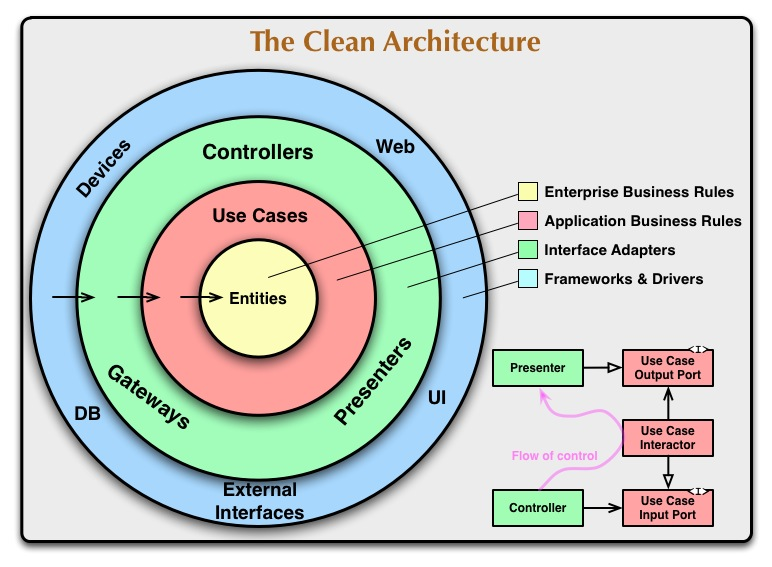
\includegraphics[width=0.8\textwidth]{figuras/clean_arch_1.jpg}
            \caption{A arquitetura limpa}
            \label{fig:figura_clean_arch_1}
            \newcommand{\source}{Fonte: \cite{livro:martin:cleanarch}}
        \end{figure}
        
        \subsubsection{Regra da Dependência}
        
            \par A Regra da Dependência é uma regra que visa estabelecer como as dependências devem se relacionar na arquitetura limpa. Ela define que dependências do código-fonte devem apontar para camadas internas, garantindo que nada em uma camada externa seja conhecido pelas camadas internas, incluindo funções, classes ou formatos de dados \cite{livro:martin:cleanarch}. 

            \par Nesse sentido, para realizar a implementação dessa regra é necessário o uso de interface abstratas, que isolam as camadas internas (entidades e casos de uso) dos detalher técnicos mais externo, como bancos de dados ou frameworks \cite{livro:martin:cleanarch}.

        \subsubsection{Entidades}
            \par As entidades são os componentes da arquitetura limpa responsáveis por encapsular as regras de negócio do software, sendo objetos ou coleções de dados e funções de tecnologias externas \cite{livro:martin:cleanarch, artigo:ferreira:2022, artigo:dantas:2021}. Elas fazem parte da camada central, que sofrera menos mudanças ao longo do tempo, e são a representação do domínio do sistemas. Além disso  as entidades garantem estabilidade, pois elas são desenvolvidas para não serem alteradas quando houver mudanças em interfaces ou bancos de dados \cite{artigo:dantas:2021, livro:martin:cleanarch}.
            
        \subsubsection{Casos de Uso}
            \par Os casos de uso são usados para realizar a implementação das regras de negócio específicas do software, orquestrando o fluxo de dados entre as entidades e outras camadas. Eles tem a característica de serem independentes de detalhes externos, com foco na intenção do negócio e também permitem que o desenvolvimento do software seja incremental e que os testes possam ser feitos de maneira isolada. \cite{artigo:ferreira:2022, livro:martin:cleanarch}
            
        \subsubsection{Adaptadores de Interface}

            \par Os adaptadores de interface são responsáveis por converter dados de formatos internos (usado por casos de uso e entidades) e externos (como bancos de dados e APIs), eles servem para isolar os detalhes técnicos da lógica do negócio da aplicação, também são úteis para facilitar a substituição de tecnologias externas sem afetar as camadas mais internas do software \cite{livro:martin:cleanarch}. 
            
        \subsubsection{Frameworks e Drivers}

            \par Os frameworks e drives representam as ferramentas e tecnologias externas, como bancos de dados, frameworks e dispositivos que fazem entrada ou saída de dados, considerado detalhes de implementação que podem mudar ao longo do tempo de desenvolvimento dos projetos \cite{livro:martin:cleanarch}.